\colorlet{species background color}{black!15}
\tikzset{
    x={1pt},
    y={-1pt},
    species border/.style={
        line width={1pt},
        shorten <={-1pt / 2 + 0.05pt},
        shorten >={-1pt / 2 + 0.05pt},
    },
    species background/.style={
        fill=species background color,
        draw=species background color,
        line width={1pt},
        rounded corners,
    },
    species label/.style={
        font=\bfseries,
        midway,
        anchor=north,
        align=center,
        yshift=-10,
    },
    branch/.style={
        draw={#1},
        line width={0.5pt},
    },
    transfer branch/.style={
        branch={#1},
        -Stealth,
    },
    loss/.style={
        draw={#1}, cross out, thick,
        line width={0.5pt},
        inner sep=0pt,
        outer sep=0pt,
        minimum width={3},
        minimum height={3},
    },
    extant gene/.style 2 args={
        circle, fill={#1},
        outer sep=0pt, inner sep=0pt,
        minimum size={3},
        label={
            [font={\strut\color{#1}},
                align=center,
                inner xsep=0pt, inner ysep=2pt,
                outer xsep=0pt, outer ysep=0pt]
            below:#2
        },
    },
    extant gene/.default={black}{},
    branch node/.style={
        draw={#1}, fill={species background color!50!white},
        align=center,
        font={\color{#1}},
        outer sep=0pt, inner xsep=0pt, inner ysep=2pt,
        line width={0.5pt},
    },
    branch node/.default={black},
    speciation/.style={
        branch node={#1}, rectangle, rounded corners,
        inner xsep=4pt,
        minimum width={8},
        minimum height={8},
    },
    duplication/.style={
        branch node={#1}, rectangle,
        inner xsep=4pt,
        minimum width={8},
        minimum height={8},
    },
    horizontal gene transfer/.style={
        branch node={#1}, chamfered rectangle,
        chamfered rectangle sep={8 / 2.4},
        inner xsep=2pt,
        inner ysep=-1pt,
        minimum width={8},
        minimum height={8},
    },
}
\definecolor{reccolor0}{HTML}{000000}
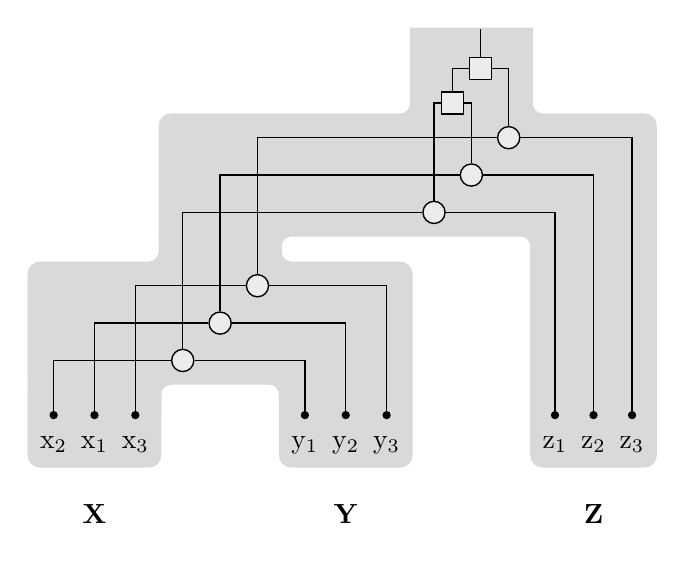
\begin{tikzpicture}
% background
\path[species background] (47.289,74.5) -- (47.289,31.0) -- (138.078,31.0) [sharp corners] -- (138.078,0) -- (181.578,0) [rounded corners] -- (181.578,31.0) -- (226.347,31.0) [sharp corners] -- (226.347,128.0) [rounded corners] -- (181.578,138.0) -- (181.578,74.5) -- (90.789,74.5) [sharp corners] -- (90.789,84.5) -- cycle;
\path[species background] (0,128.0) -- (0,84.5) -- (47.289,84.5) [sharp corners] -- (47.289,74.5) -- (90.789,74.5) [rounded corners] -- (90.789,84.5) -- (138.078,84.5) [sharp corners] -- (138.078,128.0) [rounded corners] -- (90.789,138.0) -- (90.789,128.0) -- (47.289,128.0) [sharp corners] -- (47.289,138.0) -- cycle;
\path[species background] (0,128.0) -- (0,158.0) -- (47.289,158.0) -- (47.289,128.0);
\path[species background] (90.789,128.0) -- (90.789,158.0) -- (138.078,158.0) -- (138.078,128.0);
\path[species background] (181.578,128.0) -- (181.578,158.0) -- (226.347,158.0) -- (226.347,128.0);
% species
\path[species border] (47.289,74.5) -- (47.289,31.0) -- (138.078,31.0) -- (138.078,0);
\path[species border] (226.347,128.0) -- (226.347,31.0) -- (181.578,31.0) -- (181.578,0);
\path[species border] (90.789,74.5) -- (90.789,74.5) -- (181.578,74.5) -- (181.578,128.0);
\path[species border] (0,128.0) -- (0,84.5) -- (47.289,84.5) -- (47.289,74.5);
\path[species border] (138.078,128.0) -- (138.078,84.5) -- (90.789,84.5) -- (90.789,74.5);
\path[species border] (47.289,128.0) -- (47.289,128.0) -- (90.789,128.0) -- (90.789,128.0);
\path[species border] (0,128.0) -- (0,158.0) -- node[species label] {X} (47.289,158.0) -- (47.289,128.0);
\path[species border] (90.789,128.0) -- (90.789,158.0) -- node[species label] {Y} (138.078,158.0) -- (138.078,128.0);
\path[species border] (181.578,128.0) -- (181.578,158.0) -- node[species label] {Z} (226.347,158.0) -- (226.347,128.0);
% gene branches
\draw[branch={reccolor0}] (82.539,74.5) |- (169.078,39.25) (177.578,39.25) -| (217.8855,128.0);
\draw[branch={reccolor0}] (69.039,74.5) |- (155.578,52.75) (164.078,52.75) -| (203.9625,128.0);
\draw[branch={reccolor0}] (55.539,74.5) |- (142.078,66.25) (150.578,66.25) -| (190.0395,128.0);
\draw[branch={reccolor0}] (159.828,48.5) |- (148.828,26.75) (157.328,26.75) -| (146.328,62.0);
\path[branch={reccolor0}] (163.203,10.0) -- (163.203,0);
\draw[branch={reccolor0}] (173.328,35.0) |- (158.953,14.25) (167.453,14.25) -| (153.078,22.5);
\path[branch={reccolor0}] (82.539,88.5) -- (82.539,74.5);
\draw[branch={reccolor0}] (38.4075,128.0) |- (78.289,92.75) (86.789,92.75) -| (129.19650000000001,128.0);
\path[branch={reccolor0}] (69.039,102.0) -- (69.039,74.5);
\draw[branch={reccolor0}] (23.6445,128.0) |- (64.789,106.25) (73.289,106.25) -| (114.43350000000001,128.0);
\path[branch={reccolor0}] (55.539,115.5) -- (55.539,74.5);
\draw[branch={reccolor0}] (8.881500000000003,128.0) |- (51.289,119.75) (59.789,119.75) -| (99.6705,128.0);
\path[branch={reccolor0}] (38.407500000000006,138.0) -- (38.4075,128.0);
\path[branch={reccolor0}] (23.6445,138.0) -- (23.6445,128.0);
\path[branch={reccolor0}] (8.881499999999999,138.0) -- (8.881500000000003,128.0);
\path[branch={reccolor0}] (129.1965,138.0) -- (129.19650000000001,128.0);
\path[branch={reccolor0}] (114.43350000000001,138.0) -- (114.43350000000001,128.0);
\path[branch={reccolor0}] (99.6705,138.0) -- (99.6705,128.0);
\path[branch={reccolor0}] (217.8855,138.0) -- (217.8855,128.0);
\path[branch={reccolor0}] (203.9625,138.0) -- (203.9625,128.0);
\path[branch={reccolor0}] (190.0395,138.0) -- (190.0395,128.0);
% gene transfers
% events
\node[speciation={reccolor0}] at (173.328,39.25) {};
\node[speciation={reccolor0}] at (159.828,52.75) {};
\node[speciation={reccolor0}] at (146.328,66.25) {};
\node[duplication={reccolor0}] at (153.078,26.75) {};
\node[duplication={reccolor0}] at (163.203,14.25) {};
\node[speciation={reccolor0}] at (82.539,92.75) {};
\node[speciation={reccolor0}] at (69.039,106.25) {};
\node[speciation={reccolor0}] at (55.539,119.75) {};
\node[extant gene={reccolor0}{x\textsubscript{3}}] at (38.407500000000006,139.5) {};
\node[extant gene={reccolor0}{x\textsubscript{1}}] at (23.6445,139.5) {};
\node[extant gene={reccolor0}{x\textsubscript{2}}] at (8.881499999999999,139.5) {};
\node[extant gene={reccolor0}{y\textsubscript{3}}] at (129.1965,139.5) {};
\node[extant gene={reccolor0}{y\textsubscript{2}}] at (114.43350000000001,139.5) {};
\node[extant gene={reccolor0}{y\textsubscript{1}}] at (99.6705,139.5) {};
\node[extant gene={reccolor0}{z\textsubscript{3}}] at (217.8855,139.5) {};
\node[extant gene={reccolor0}{z\textsubscript{2}}] at (203.9625,139.5) {};
\node[extant gene={reccolor0}{z\textsubscript{1}}] at (190.0395,139.5) {};
\end{tikzpicture}
